% Options for packages loaded elsewhere
\PassOptionsToPackage{unicode}{hyperref}
\PassOptionsToPackage{hyphens}{url}
%
\documentclass[
]{compterendu}
\usepackage{amsmath,amssymb}
\usepackage{iftex}
\ifPDFTeX
  \usepackage[T1]{fontenc}
  \usepackage[utf8]{inputenc}
  \usepackage{textcomp} % provide euro and other symbols
\else % if luatex or xetex
  \usepackage{unicode-math} % this also loads fontspec
  \defaultfontfeatures{Scale=MatchLowercase}
  \defaultfontfeatures[\rmfamily]{Ligatures=TeX,Scale=1}
\fi
\usepackage{lmodern}
\ifPDFTeX\else
  % xetex/luatex font selection
\fi
% Use upquote if available, for straight quotes in verbatim environments
\IfFileExists{upquote.sty}{\usepackage{upquote}}{}
\IfFileExists{microtype.sty}{% use microtype if available
  \usepackage[]{microtype}
  \UseMicrotypeSet[protrusion]{basicmath} % disable protrusion for tt fonts
}{}
\makeatletter
\@ifundefined{KOMAClassName}{% if non-KOMA class
  \IfFileExists{parskip.sty}{%
    \usepackage{parskip}
  }{% else
    \setlength{\parindent}{0pt}
    \setlength{\parskip}{6pt plus 2pt minus 1pt}}
}{% if KOMA class
  \KOMAoptions{parskip=half}}
\makeatother
\usepackage{xcolor}
\usepackage[left=2cm,right=2cm,top=2.5cm,bottom=2.5cm]{geometry}
\usepackage{longtable,booktabs,array}
\usepackage{calc} % for calculating minipage widths
% Correct order of tables after \paragraph or \subparagraph
\usepackage{etoolbox}
\makeatletter
\patchcmd\longtable{\par}{\if@noskipsec\mbox{}\fi\par}{}{}
\makeatother
% Allow footnotes in longtable head/foot
\IfFileExists{footnotehyper.sty}{\usepackage{footnotehyper}}{\usepackage{footnote}}
\makesavenoteenv{longtable}
\usepackage{graphicx}
\makeatletter
\def\maxwidth{\ifdim\Gin@nat@width>\linewidth\linewidth\else\Gin@nat@width\fi}
\def\maxheight{\ifdim\Gin@nat@height>\textheight\textheight\else\Gin@nat@height\fi}
\makeatother
% Scale images if necessary, so that they will not overflow the page
% margins by default, and it is still possible to overwrite the defaults
% using explicit options in \includegraphics[width, height, ...]{}
\setkeys{Gin}{width=\maxwidth,height=\maxheight,keepaspectratio}
% Set default figure placement to htbp
\makeatletter
\def\fps@figure{htbp}
\makeatother
\setlength{\emergencystretch}{3em} % prevent overfull lines
\providecommand{\tightlist}{%
  \setlength{\itemsep}{0pt}\setlength{\parskip}{0pt}}
\setcounter{secnumdepth}{-\maxdimen} % remove section numbering
\ifLuaTeX
\usepackage[bidi=basic]{babel}
\else
\usepackage[bidi=default]{babel}
\fi
\babelprovide[main,import]{french}
% get rid of language-specific shorthands (see #6817):
\let\LanguageShortHands\languageshorthands
\def\languageshorthands#1{}
\usepackage{booktabs}
\usepackage{longtable}
\usepackage{array}
\usepackage{multirow}
\usepackage{wrapfig}
\usepackage{float}
\usepackage{colortbl}
\usepackage{pdflscape}
\usepackage{tabu}
\usepackage{threeparttable}
\usepackage{threeparttablex}
\usepackage[normalem]{ulem}
\usepackage{makecell}
\usepackage{xcolor}
\ifLuaTeX
  \usepackage{selnolig}  % disable illegal ligatures
\fi
\usepackage{bookmark}
\IfFileExists{xurl.sty}{\usepackage{xurl}}{} % add URL line breaks if available
\urlstyle{same}
\hypersetup{
  pdftitle={Analyse des données sur les infrastructures aéroportuaires},
  pdfauthor={Ismaël Madou Gagi Grema; Nikita Pomozov},
  pdflang={true},
  hidelinks,
  pdfcreator={LaTeX via pandoc}}

\title{Analyse des données sur les infrastructures aéroportuaires}
\author{Ismaël Madou Gagi Grema \and Nikita Pomozov}
\date{2024-12-18}

\begin{document}
\maketitle
\begin{abstract}
La problématique est d'appréhender l'impact du revenu national sur les
infrastructures aéroportuaires ainsi que les choix des différents pays
dans le développement des infrastructures aéroportuaires.
\end{abstract}

{
\setcounter{tocdepth}{2}
\tableofcontents
}
\section{\texorpdfstring{\textbf{Les acronyms des pays utilisés pour
l'analyse}}{Les acronyms des pays utilisés pour l'analyse}}\label{les-acronyms-des-pays-utilisuxe9s-pour-lanalyse}

\subsubsection{Pays}\label{pays}

\begin{longtable}[]{@{}ll@{}}
\toprule\noalign{}
Acronyme & Pays \\
\midrule\noalign{}
\endhead
\bottomrule\noalign{}
\endlastfoot
AE & Emirats Arabes Unis \\
BR & Brésil \\
CA & Canada \\
CN & Chine \\
JP & Japon \\
KR & Corée du Sud \\
US & États-Unis \\
\end{longtable}

\subsubsection{Types d'aéroports}\label{types-dauxe9roports}

\begin{longtable}[]{@{}ll@{}}
\toprule\noalign{}
Acronyme & Type d'aéroport \\
\midrule\noalign{}
\endhead
\bottomrule\noalign{}
\endlastfoot
Small\_airports & Petit aéroport \\
medium\_airport & Moyen aéroport \\
large\_airport & Grand aéroport \\
heliport & Héliport \\
closed & Fermé \\
balloonport & Port de ballons \\
seaplane\_base & Base d'hydravions \\
\end{longtable}

\section{\texorpdfstring{\textbf{Introduction}}{Introduction}}\label{introduction}

Les aéroports jouent un rôle central dans le transport aérien mondial,
facilitant les échanges internationaux, le tourisme, les affaires et le
commerce. En tant qu'infrastructures stratégiques, leur gestion et leur
développement sont essentiels pour les économies locales et mondiales.

Cette étude se concentre sur une base de données regroupant des
informations détaillées sur les aéroports du monde, incluant leur
localisation, leur type et leurs caractéristiques, répartis à travers
différents pays.

À travers cette analyse, nous explorerons des variables clés telles que
le type d'aéroport (grands, petits, moyens, héliports, etc.) et les
codes ISO des pays en utilisant la méthode d'AFC, afin de comprendre les
choix des pays dans le développement des infrastructures aéroportuaires.
D'autre part, nous étudierons des variables telles que le revenu
national (provenant d'une autre base de données fusionnée avec la
présente base), le nombre de passagers, la longueur des pistes ainsi que
leur largeur, en utilisant la méthode de l'ACP pour évaluer l'impact des
revenus nationaux sur le développement de ces infrastructures.

La problématique est de comprendre les choix des pays dans la
construction des infrastructures aéroportuaires, mais également
d'analyser l'impact des revenus nationaux sur la mise en œuvre de ces
infrastructures. Cela nous permettra de déterminer si les pays les plus
riches investissent davantage dans les aéroports et si cela se traduit
par une augmentation du nombre de passagers.

\section{\texorpdfstring{\textbf{Section 1: les choix des pays dans le
developpement des
infrastructures}}{Section 1: les choix des pays dans le developpement des infrastructures}}\label{section-1-les-choix-des-pays-dans-le-developpement-des-infrastructures}

À ce niveau, nous avons regroupé les pays ayant un nombre d'aéroports
inférieur à 200 dans une classe appelée ``autres''. Cela nous donne,
dans ce cas, 38 pays au lieu de 245. Cette modification a été réalisée
suite à une remarque de M. Regnault, qui a souligné que l'AFC tend à
biaiser les résultats en attribuant un poids disproportionné aux pays
ayant un faible nombre d'aéroports.

Le choix des pays dans le développement des infrastructures
aéroportuaires dépend de plusieurs facteurs, qui peuvent être liés à
l'économie, à la politique, à la géopolitique, mais aussi à des raisons
purement sociales. Les pays développés ou à revenu élevé investissent
généralement massivement dans leurs infrastructures aéroportuaires en
raison de leur forte demande de transport aérien et de leur rôle central
dans le commerce mondial.

Par exemple, des pays comme la Chine et les États-Unis, d'après les
résultats de nos analyses, possèdent un grand nombre de moyens aéroports
en raison de plusieurs facteurs. Leur vaste taille géographique et leur
population importante génèrent une forte demande pour un réseau aérien
étendu.

Les États-Unis, avec une économie développée et une politique de
décentralisation, disposent de nombreux aéroports régionaux pour
desservir des villes moyennes et petites. En Chine, l'urbanisation
rapide et la croissance économique ont conduit à la construction
d'aéroports dans des régions moins accessibles. Ces deux pays
investissent massivement dans les infrastructures pour connecter
efficacement leurs vastes territoires.

Le tourisme international et les échanges commerciaux renforcent
également la nécessité de ces aéroports. Grâce à leur réseau aérien
dense, les États-Unis et la Chine facilitent les déplacements internes
et internationaux. Enfin, le développement rapide de la Chine au cours
des dernières décennies a particulièrement accentué cette dynamique.

Le nombre élevé d'héliports en Corée du Sud et au Japon s'explique par
plusieurs facteurs. Ces pays, fortement urbanisés, présentent une
densité de population élevée dans leurs grandes villes, telles que Tokyo
et Séoul, où l'espace est limité. Les hélicoptères offrent une solution
de transport rapide et flexible, particulièrement utile dans les zones
difficiles d'accès.

La géographie particulière de ces pays, notamment les montagnes et les
nombreuses îles du Japon, rend l'utilisation des infrastructures
terrestres coûteuse et complexe. Les héliports permettent de faciliter
l'accès aux zones rurales ou isolées. Par ailleurs, ces nations sont
fréquemment confrontées à des catastrophes naturelles, ce qui rend les
hélicoptères indispensables pour les opérations de secours d'urgence.

Le Japon et la Corée du Sud ont également investi dans des technologies
de pointe pour améliorer la sécurité et l'efficacité de ces
infrastructures. Les héliports sont utilisés à des fins variées,
notamment commerciales, médicales et militaires. Enfin, la forte demande
de services aériens dans des environnements urbains densément peuplés
renforce leur développement et leur utilisation.

Le nombre élevé d'aéroports fermés et d'hydravions au Canada et au
Brésil s'explique par des facteurs géographiques et logistiques. Ces
deux pays, caractérisés par leur immense territoire, comptent de
nombreuses régions isolées et difficiles d'accès par voie terrestre.

En raison de la faible densité de population dans certaines zones et des
coûts élevés pour maintenir des infrastructures aériennes, de nombreux
petits aéroports ont été fermés. Les hydravions, en revanche, offrent
une solution pratique et économique pour relier ces régions reculées. Au
Canada, ils sont particulièrement adaptés aux conditions géographiques,
comme les lacs et rivières, tandis qu'au Brésil, ils jouent un rôle
crucial dans l'Amazonie, où le réseau routier est limité.

Ces aéronefs permettent de desservir efficacement les communautés
isolées tout en s'intégrant aux contraintes géographiques locales. Au
Canada, les hydravions sont également largement utilisés pour des
services de transport et d'urgence dans des zones difficiles d'accès.
Ainsi, dans les deux pays, les hydravions remplacent efficacement les
petits aéroports fermés, offrant une solution aérienne plus flexible et
adaptée aux besoins locaux.

De plus, nous avons observé que certains États, comme les États-Unis et
la Chine, possèdent des proportions similaires de différents types
d'aéroports, reflétant la diversité de leurs besoins en transport. Les
grands aéroports sont principalement destinés aux voyages
internationaux, tandis que les aéroports moyens et petits répondent aux
déplacements domestiques ou régionaux.

Dans des pays vastes et géographiquement variés, cette diversité est
essentielle pour connecter efficacement les zones urbaines, rurales et
isolées. Elle permet également de répondre à des besoins spécifiques,
tels que le transport d'urgence ou l'accès à des régions éloignées.
Cette combinaison assure une couverture complète et flexible du réseau
aérien, adaptée à des contextes variés et à des enjeux économiques,
sociaux et géographiques.

\section{\texorpdfstring{\textbf{Section 2: L'impact des revenus
nationaux sur les infrastructures
aeroportuaires}}{Section 2: L'impact des revenus nationaux sur les infrastructures aeroportuaires}}\label{section-2-limpact-des-revenus-nationaux-sur-les-infrastructures-aeroportuaires}

Pour analyser l'impact des revenus nationaux sur les infrastructures
aéroportuaires, nous avons combiné plusieurs ensembles de données. Cela
inclut des informations sur les aéroports (localisation, taille et
caractéristiques), les codes ISO des pays (utilisés comme clés pour
fusionner les ensembles), les revenus nationaux par habitant (comme
indicateur de la richesse économique) et le trafic annuel de passagers
des 50 principaux aéroports (extraits de Wikipedia en raison de
limitations d'accès aux données complètes sur tous les aéroports).

En utilisant des variables comme les revenus nationaux, la longueur et
la largeur des pistes, ainsi que le nombre de passagers, nous avons
cherché à comprendre les relations entre ces facteurs pour déterminer si
les pays les plus riches investissent davantage dans leurs aéroports et
si ces investissements se traduisent par un trafic aérien accru.

L'analyse visuelle montre des différences notables entre les 50
principaux aéroports mondiaux et les 75 000 aéroports dans leur
ensemble. Les grandes infrastructures, comme des pistes plus longues et
plus larges, sont principalement concentrées dans ces grands aéroports.
Cela s'explique par plusieurs observations : - Les pistes plus longues
sont nécessaires pour accueillir des avions transcontinentaux, qui
nécessitent des distances supplémentaires pour décoller et atterrir. -
Ces grands aéroports agissent comme des hubs internationaux, nécessitant
des investissements massifs dans les infrastructures pour répondre aux
flux croissants de passagers et de marchandises.

Les données confirment que les pays les plus riches tendent à développer
de grandes infrastructures aéroportuaires pour répondre à une demande
accrue en transport aérien. Cependant, certaines exceptions
apparaissent, révélant des schémas intéressants : - Certains pays à
revenu limité enregistrent un trafic élevé, souvent grâce à leur rôle de
hubs régionaux ou à leur dépendance au tourisme, comme les Maldives ou
des pays d'Afrique de l'Est. - À l'inverse, certains pays comme le
Bresil et la Chine disposant d'infrastructures avancées affichent un
trafic passagers relativement faible, ce qui pourrait indiquer des
inefficacités dans la gestion de ces aéroports ou une faible demande due
à des facteurs économiques, sociaux ou géopolitiques.

Notre analyse a été limitée par l'accès restreint aux données détaillées
sur l'ensemble des aéroports mondiaux. En conséquence, les conclusions
actuelles s'appuient principalement sur les 50 top aéroports. Pour une
compréhension plus complète des tendances, il serait essentiel de
disposer de données couvrant une plus large gamme d'aéroports, y compris
ceux situés dans des pays en développement ou dans des régions peu
accessibles.

\section{\texorpdfstring{\textbf{Conclusion}}{Conclusion}}\label{conclusion}

Les résultats de l'analyse mettent en évidence une relation complexe
entre la richesse nationale, les infrastructures aéroportuaires et le
transport aérien. Si les pays les plus riches investissent généralement
davantage dans leurs infrastructures aéroportuaires, ce qui se traduit
par des volumes de trafic plus élevés, certaines exceptions notables
suggèrent l'influence de facteurs supplémentaires.

Des éléments tels que la localisation géographique, les politiques
publiques, la connectivité aérienne ou encore la dépendance au tourisme
jouent un rôle déterminant dans ces variations. Ces facteurs soulignent
la nécessité d'examiner de manière approfondie les anomalies et les
écarts par rapport au schéma général, afin de mieux comprendre la
dynamique complexe entre le développement économique, les
infrastructures aéroportuaires et les flux de passagers.

Pour aller plus loin, une analyse détaillée des outliers et des facteurs
externes s'avère indispensable. De plus, l'utilisation d'un ensemble de
données plus exhaustif, incluant un plus grand nombre d'aéroports,
serait cruciale pour confirmer ces observations et affiner les
conclusions.

En résumé, le développement des infrastructures aéroportuaires reflète
souvent des choix stratégiques basés sur des besoins spécifiques propres
à chaque pays. Ces décisions résultent d'une combinaison de facteurs
économiques, politiques et sociaux, permettant aux nations d'adapter
leurs investissements pour répondre aux exigences de leurs territoires
et de leurs populations.

\section{\texorpdfstring{\textbf{Annexe}}{Annexe}}\label{annexe}

\subsection{L'AFC}\label{lafc}

L'AFC (Analyse Factorielle des Correspondances) est une méthode
statistique exploratoire utilisée pour analyser des tableaux de
contingence, généralement dans le cadre de variables qualitatives. Elle
permet de visualiser et d'interpréter les relations entre les lignes et
les colonnes d'un tableau de contingence. Dans notre cas, nous allons
analyser le tableau de contingence avec les différents pays représentés
en ligne et les types d'aéroports en colonne.

La première partie de notre méthode d'AFC concerne l'analyse
descriptive. Cette analyse descriptive nous permettra de résumer de
façon simple et concise l'ensemble des données.

L'analyse univariée se concentre sur l'étude d'une seule variable à la
fois, qu'elle soit quantitative ou qualitative. L'objectif de cette
analyse est de décrire les caractéristiques de la variable et de
comprendre sa distribution. Elle permet d'obtenir une première idée de
la structure des données avant de passer à une analyse bivariée ou
multivariée.

\begin{table}

\caption{\label{tab:tableex}Tableau des statistiques descriptives}
\centering
\begin{tabular}[t]{lllllllllllllllllllllllllllll}
\toprule
  &       X &       Y &    OBJECTID &       id & airport\_ident &     type &     name & latitude\_deg & longitude\_deg &  elevation\_ft &  continent & iso\_country &  iso\_region & municipality & scheduled\_service &   gps\_code &  iata\_code &  local\_code &  home\_link & wikipedia\_link &   keywords & description & frequency\_mhz & runway\_length\_ft & runway\_width\_ft & runway\_surface & runway\_lighted & runway\_closed\\
\midrule
 & Min.   :-20023816 & Min.   :-15743333 & Min.   :    1 & Min.   :     2 & Length:75052 & Length:75052 & Length:75052 & Length:75052 & Min.   :-179.88 & Min.   :-1266 & Length:75052 & Length:75052 & Length:75052 & Length:75052 & Length:75052 & Length:75052 & Length:75052 & Length:75052 & Length:75052 & Length:75052 & Length:75052 & Length:75052 & Min.   :   0.0 & Min.   :    0 & Min.   :   0.0 & Length:75052 & Min.   :0.00 & Min.   :0.00\\
 & 1st Qu.:-10473682 & 1st Qu.:  1269899 & 1st Qu.:18764 & 1st Qu.: 18910 & Class :character & Class :character & Class :character & Class :character & 1st Qu.: -94.09 & 1st Qu.:  205 & Class :character & Class :character & Class :character & Class :character & Class :character & Class :character & Class :character & Class :character & Class :character & Class :character & Class :character & Class :character & 1st Qu.: 120.1 & 1st Qu.: 1500 & 1st Qu.:  59.0 & Class :character & 1st Qu.:0.00 & 1st Qu.:0.00\\
 & Median : -7723717 & Median :  4180065 & Median :37526 & Median : 40240 & Mode  :character & Mode  :character & Mode  :character & Mode  :character & Median : -69.38 & Median :  730 & Mode  :character & Mode  :character & Mode  :character & Mode  :character & Mode  :character & Mode  :character & Mode  :character & Mode  :character & Mode  :character & Mode  :character & Mode  :character & Mode  :character & Median : 122.9 & Median : 2622 & Median :  75.0 & Mode  :character & Median :0.00 & Median :0.00\\
 & Mean   : -3188512 & Mean   :  3214841 & Mean   :37526 & Mean   :156747 & NA & NA & NA & NA & Mean   : -28.64 & Mean   : 1301 & NA & NA & NA & NA & NA & NA & NA & NA & NA & NA & NA & NA & Mean   : 131.5 & Mean   : 3050 & Mean   : 103.8 & NA & Mean   :0.23 & Mean   :0.01\\
 & 3rd Qu.:  2715492 & 3rd Qu.:  5260454 & 3rd Qu.:56289 & 3rd Qu.:334350 & NA & NA & NA & NA & 3rd Qu.:  24.39 & 3rd Qu.: 1613 & NA & NA & NA & NA & NA & NA & NA & NA & NA & NA & NA & NA & 3rd Qu.: 126.7 & 3rd Qu.: 3999 & 3rd Qu.: 100.0 & NA & 3rd Qu.:0.00 & 3rd Qu.:0.00\\
\addlinespace
 & Max.   : 20034803 & Max.   : 17597517 & Max.   :75052 & Max.   :508396 & NA & NA & NA & NA & Max.   : 179.98 & Max.   :17372 & NA & NA & NA & NA & NA & NA & NA & NA & NA & NA & NA & NA & Max.   :1340.0 & Max.   :30000 & Max.   :9000.0 & NA & Max.   :1.00 & Max.   :1.00\\
 & NA's   :1 & NA's   :1 & NA & NA & NA & NA & NA & NA & NA & NA's   :14263 & NA & NA & NA & NA & NA & NA & NA & NA & NA & NA & NA & NA & NA's   :64383 & NA's   :37241 & NA's   :39483 & NA & NA's   :37062 & NA's   :37062\\
\bottomrule
\end{tabular}
\end{table}

\begin{table}[!h]
\centering
\caption{\label{tab:unnamed-chunk-4}Nombre de valeurs manquantes par colonne}
\centering
\begin{tabular}[t]{l|r}
\hline
\textbf{ } & \textbf{x}\\
\hline
\cellcolor{gray!10}{X} & \cellcolor{gray!10}{1}\\
\hline
Y & 1\\
\hline
\cellcolor{gray!10}{OBJECTID} & \cellcolor{gray!10}{0}\\
\hline
id & 0\\
\hline
\cellcolor{gray!10}{airport\_ident} & \cellcolor{gray!10}{0}\\
\hline
type & 0\\
\hline
\cellcolor{gray!10}{name} & \cellcolor{gray!10}{0}\\
\hline
latitude\_deg & 0\\
\hline
\cellcolor{gray!10}{longitude\_deg} & \cellcolor{gray!10}{0}\\
\hline
elevation\_ft & 14263\\
\hline
\cellcolor{gray!10}{continent} & \cellcolor{gray!10}{36226}\\
\hline
iso\_country & 259\\
\hline
\cellcolor{gray!10}{iso\_region} & \cellcolor{gray!10}{0}\\
\hline
municipality & 0\\
\hline
\cellcolor{gray!10}{scheduled\_service} & \cellcolor{gray!10}{0}\\
\hline
gps\_code & 0\\
\hline
\cellcolor{gray!10}{iata\_code} & \cellcolor{gray!10}{0}\\
\hline
local\_code & 0\\
\hline
\cellcolor{gray!10}{home\_link} & \cellcolor{gray!10}{0}\\
\hline
wikipedia\_link & 0\\
\hline
\cellcolor{gray!10}{keywords} & \cellcolor{gray!10}{0}\\
\hline
description & 0\\
\hline
\cellcolor{gray!10}{frequency\_mhz} & \cellcolor{gray!10}{64383}\\
\hline
runway\_length\_ft & 37241\\
\hline
\cellcolor{gray!10}{runway\_width\_ft} & \cellcolor{gray!10}{39483}\\
\hline
runway\_surface & 0\\
\hline
\cellcolor{gray!10}{runway\_lighted} & \cellcolor{gray!10}{37062}\\
\hline
runway\_closed & 37062\\
\hline
\end{tabular}
\end{table}

Les résultats montrent que presque toutes les variables n'ont pas de
valeurs manquantes, à l'exception de X, Y, frequency,
runway\_length\_ft, runway\_width\_ft, runway\_lighted et
runway\_closed. Pour notre part, nous nous concentrerons sur des
variables telles que ``iso\_country''.

\begin{verbatim}
## 
##    balloonport         closed       heliport  large_airport medium_airport 
##             45          10164          19080            464           4747 
##  seaplane_base  small_airport 
##           1133          39419
\end{verbatim}

La première variable comporte sept types d'aéroports. Le nombre
d'occurrences de chaque type d'aéroport varie d'un pays à l'autre en
fonction des choix stratégiques de ces derniers. Les pays ayant des
orientations commerciales ont tendance à développer des aéroports
petits, moyens et grands, contrairement aux pays ayant d'autres
priorités.

Ensuite, nous allons présenter les graphiques des variables que nous
avons retenues pour effectuer l'AFC, à savoir le type d'aéroport et le
pays.

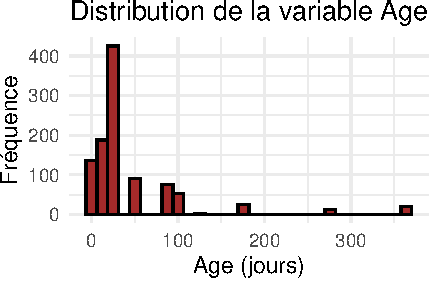
\includegraphics{rmarkdown_airportsv2_files/figure-latex/unnamed-chunk-7-1.pdf}

Ce graphique nous renseigne sur la fréquence des différents types
d'aéroports. Les petits aéroports sont les plus nombreux et représentent
la plus grande partie de notre base de données. Viennent ensuite les
héliports, avec une proportion moins importante. Puis, suivent les
aéroports moyens, et enfin, les autres types d'aéroports, qui ont une
faible proportion.

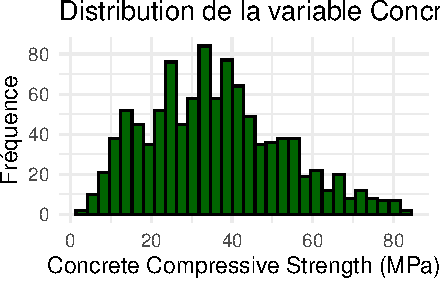
\includegraphics{rmarkdown_airportsv2_files/figure-latex/unnamed-chunk-8-1.pdf}

À ce niveau, on constate que les aéroports américains apparaissent très
fréquemment, avec plus de 25 000 aéroports. Cela signifie que les
États-Unis possèdent un nombre d'aéroports bien plus élevé que les
autres pays, dont le nombre se situe généralement entre 0 et 5 000.

L'analyse bivariée est une méthode statistique utilisée pour examiner la
relation entre deux variables. Dans ce cas, nous allons étudier la
relation entre les variables ``type'' et ``iso\_country''.

\begin{verbatim}
## 
##     AE     AR     AU Autres     BO     BR     CA     CD     CL     CN     CO 
##      1      1      1    207      1      1      1      1      1      1      1 
##     CZ     DE     ES     FR     GB     ID     IN     IR     IT     JP     KE 
##      1      1      1      1      1      1      1      1      1      1      1 
##     KR     MX     NO     NZ     PG     PH     PL     PT     RU     SE     TR 
##      1      1      1      1      1      1      1      1      1      1      1 
##     TZ     UA     US     VE     ZA 
##      1      1      1      1      1
\end{verbatim}

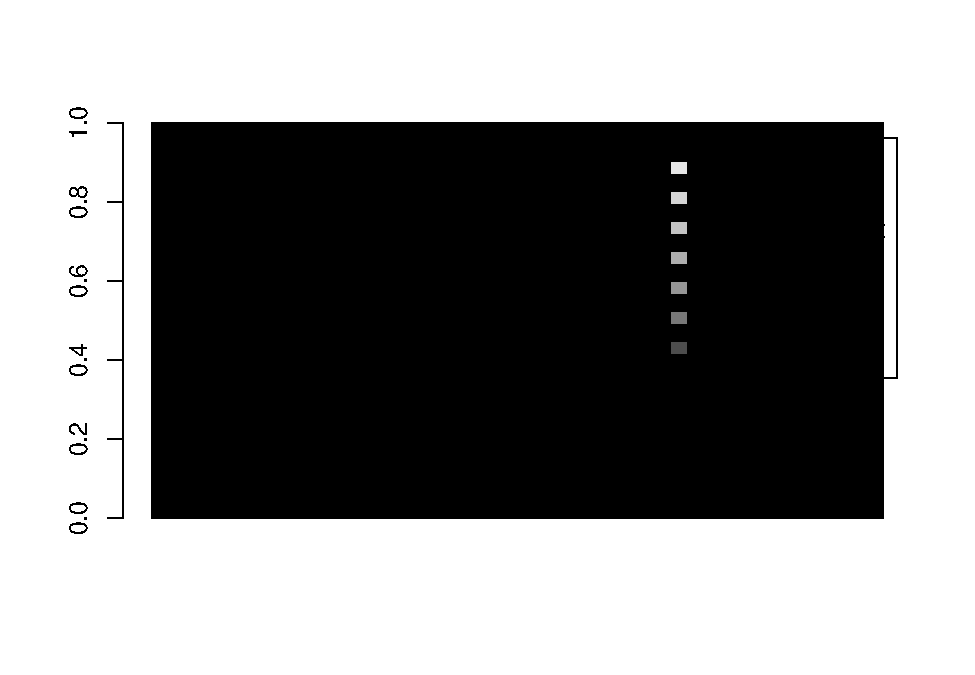
\includegraphics{rmarkdown_airportsv2_files/figure-latex/unnamed-chunk-10-1.pdf}

On constate une faible corrélation entre les aéroports fermés, les
héliports d'une part, et les grands aéroports d'autre part. Cependant,
il existe une corrélation moyenne entre les hydravions et les grands
aéroports. De plus, une corrélation modérée est observée entre les
petits et les grands aéroports, bien que cette corrélation ne soit pas
très forte.

Il convient également de noter une corrélation faible entre les
hydravions et les moyens aéroports. Une corrélation modérée existe aussi
entre les aéroports moyens, d'une part, et les héliports ainsi que les
aéroports fermés.

Cela pourrait refléter la diversité des fonctions de ces aéroports (vols
commerciaux, services régionaux, activités spécialisées, etc.). Il est
probable que des facteurs géographiques, économiques et techniques
jouent un rôle important dans la manière dont ces types d'aéroports sont
interconnectés. Les grandes infrastructures (grands aéroports) semblent
être relativement indépendantes des autres types d'infrastructures
aéronautiques, tandis que des corrélations modérées existent entre
certains types d'aéroports plus petits et spécifiques (héliports,
aéroports fermés, etc.).

Pearson's Chi-squared test

data: tableau\_croise X-squared = 30863, df = 1458, p-value \textless{}
2.2e-16

Étant donné que la p-value est inférieure à 0,05, nous rejetons
l'hypothèse nulle. Cela signifie qu'il existe une relation significative
entre les deux variables qualitatives que nous avons testées. En
d'autres termes, les résultats suggèrent que le type d'aéroport et le
pays (ou le code ISO du pays) sont liés d'une manière statistiquement
significative, et cette relation mérite d'être explorée davantage.

Fisher's Exact Test for Count Data with simulated p-value (based on
10000 replicates)

data: tableau\_croise p-value = 9.999e-05 alternative hypothesis:
two.sided

Cela signifie que le test de Fisher examine une association bilatérale,
c'est-à-dire qu'il teste si les deux variables sont significativement
liées, sans spécifier à priori une direction particulière pour
l'association.

\begin{verbatim}
##                    X^2   df P(> X^2)
## Likelihood Ratio 26501 1458        0
## Pearson          30863 1458        0
## 
## Phi-Coefficient   : NA 
## Contingency Coeff.: 0.54 
## Cramer's V        : 0.262
\end{verbatim}

Nous constatons une p-value faible, ce qui signifie qu'il existe une
forte corrélation entre les deux variables qualitatives. De plus, les
variables ``coefficient de contingence'' et ``V de Cramér'' indiquent
une association modérée.

\begin{verbatim}
## Warning in chisq.test(tableau_contingence_no_iso): Chi-squared approximation
## may be incorrect
\end{verbatim}

\begin{verbatim}
## X-squared 
##  23537.67
\end{verbatim}

\begin{verbatim}
## X-squared 
##  1.314704
\end{verbatim}

Avec une statistique χ² de 30863,32 et une p-value proche de 0, vous
pouvez conclure qu'il existe une forte association entre les deux
variables catégorielles étudiées. Cette association nous permet
d'expliquer l'une des variables en fonction de l'autre, ce qui améliore
la compréhension.

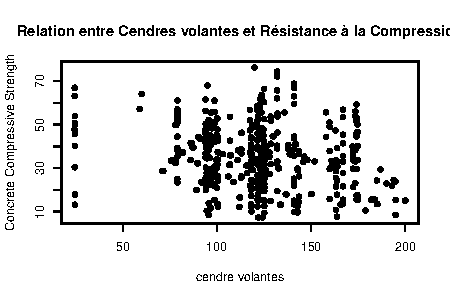
\includegraphics{rmarkdown_airportsv2_files/figure-latex/unnamed-chunk-16-1.pdf}

À ce niveau, nous avons un graphique qui indique la répartition des
types d'aéroports pour chaque pays.

Pour les petits aéroports, nous avons en première position le Kenya,
suivi de la Tanzanie, puis de la Bolivie et de l'Afrique du Sud.
Globalement, on remarque que les petits aéroports sont plus nombreux que
les autres types d'aéroports.

Concernant les hydravions, leur nombre est relativement faible.
Cependant, nous constatons que le Canada semble développer ce type
d'aéroports plus que n'importe quel autre pays.

En ce qui concerne les moyens aéroports, la Chine se distingue par le
plus grand nombre de ce type d'aéroports parmi tous les pays.

De plus, le Japon, la Turquie, la Corée du Sud et les Émirats Arabes
Unis ont tendance à développer davantage les héliports.

Les grands aéroports sont concentrés dans des pays comme la Chine, la
Norvège et la Turquie.

Enfin, nous constatons que des pays comme l'Ukraine, la Grande-Bretagne,
le Canada et les États-Unis ont fermé de nombreux aéroports, notamment
en raison de plusieurs facteurs.

Cependant, nous ne pouvons rien dire concernant les ports de ballons.

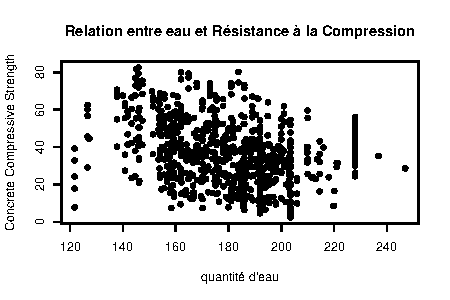
\includegraphics{rmarkdown_airportsv2_files/figure-latex/unnamed-chunk-18-1.pdf}

Ce barplot des profils de lignes indique la répartition de chaque type
d'aéroport en fonction du pays.

On remarque qu'un nombre limité de pays possèdent des ballonports, des
héliports et des hydravions. Cependant, pour les autres types
d'aéroports, l'occurrence est présente dans presque tous les pays.

Par ailleurs, nous notons également que certains pays ont une fréquence
plus élevée que celle des autres pays pour les types d'aéroports les
plus fréquents.

\begin{verbatim}
## **Results of the Correspondence Analysis (CA)**
## The row variable has  38  categories; the column variable has 7 categories
## The chi square of independence between the two variables is equal to 23537.67 (p-value =  0 ).
## *The results are available in the following objects:
## 
##    name              description                   
## 1  "$eig"            "eigenvalues"                 
## 2  "$col"            "results for the columns"     
## 3  "$col$coord"      "coord. for the columns"      
## 4  "$col$cos2"       "cos2 for the columns"        
## 5  "$col$contrib"    "contributions of the columns"
## 6  "$row"            "results for the rows"        
## 7  "$row$coord"      "coord. for the rows"         
## 8  "$row$cos2"       "cos2 for the rows"           
## 9  "$row$contrib"    "contributions of the rows"   
## 10 "$call"           "summary called parameters"   
## 11 "$call$marge.col" "weights of the columns"      
## 12 "$call$marge.row" "weights of the rows"
\end{verbatim}

\begin{verbatim}
##         eigenvalue percentage of variance cumulative percentage of variance
## dim 1 0.1655988661            52.62047396                          52.62047
## dim 2 0.0679060590            21.57773838                          74.19821
## dim 3 0.0632976134            20.11336487                          94.31158
## dim 4 0.0161109031             5.11937900                          99.43096
## dim 5 0.0015162855             0.48181284                          99.91277
## dim 6 0.0002745195             0.08723095                         100.00000
\end{verbatim}

\begin{verbatim}
##         eigenvalue percentage of variance cumulative percentage of variance
## dim 1 0.1655988661            52.62047396                          52.62047
## dim 2 0.0679060590            21.57773838                          74.19821
## dim 3 0.0632976134            20.11336487                          94.31158
## dim 4 0.0161109031             5.11937900                          99.43096
## dim 5 0.0015162855             0.48181284                          99.91277
## dim 6 0.0002745195             0.08723095                         100.00000
\end{verbatim}

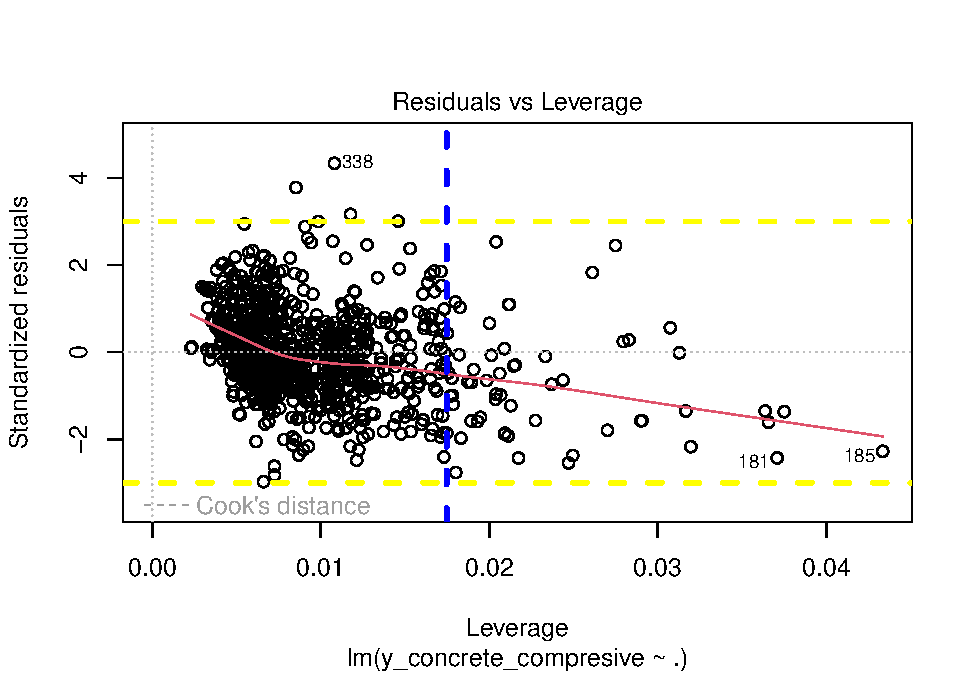
\includegraphics{rmarkdown_airportsv2_files/figure-latex/unnamed-chunk-21-1.pdf}

Ces résultats nous fournissent des informations sur les valeurs propres
ainsi que la variance expliquée, qui correspond à l'explication de la
variabilité des données observées.

Règle du coude : on retient 3 valeurs propres qui représentent 94,31 \%
de l'inertie. Cela signifie que ces trois valeurs expliquent à elles
seules la majeure partie de l'information.

\begin{verbatim}
## Warning: ggrepel: 2 unlabeled data points (too many overlaps). Consider
## increasing max.overlaps
\end{verbatim}

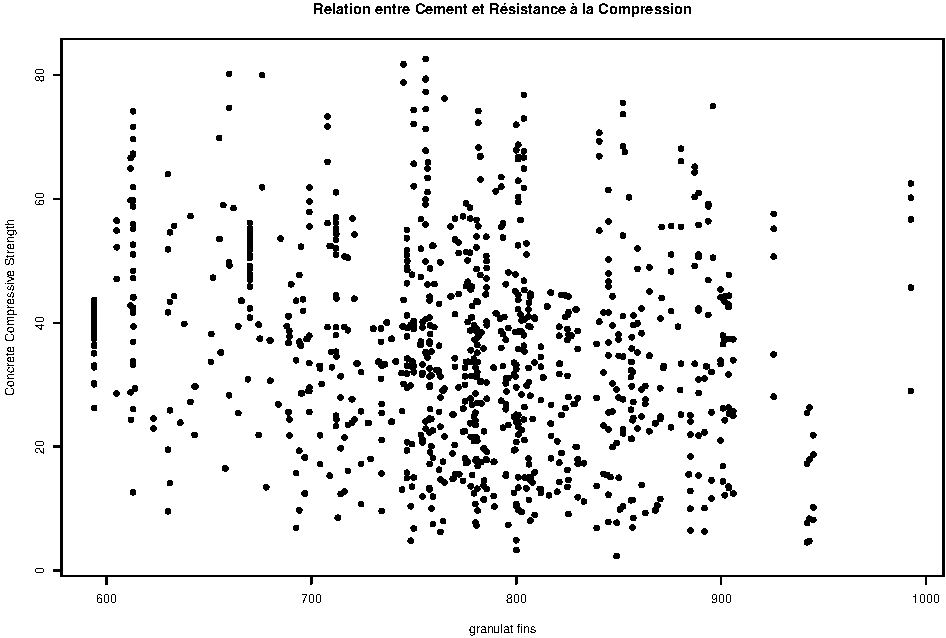
\includegraphics{rmarkdown_airportsv2_files/figure-latex/unnamed-chunk-22-1.pdf}

À ce niveau, nous nous focaliserons sur les deux premiers axes pour
analyser les données. Ces deux dimensions expliquent 74,19 \% de
l'information (variance expliquée).

Les types d'aéroports qui sont bien représentés sur le premier axe sont
les héliports (heliport) et les petits aéroports (small\_airport). De
plus, l'héliport contribue en grande partie à la construction du premier
axe, sans oublier la contribution des petits aéroports. Ce premier axe
oppose les héliports aux petits aéroports. Sur cet axe, des pays comme
le Japon et la Corée du Sud sont bien représentés et contribuent
fortement à la construction du premier axe.

Sur le second axe, on observe une opposition entre les hydravions d'une
part et les autres types d'aéroports d'autre part. Les hydravions et les
aéroports fermés contribuent en grande partie à la construction du
deuxième axe et sont très bien représentés sur cet axe. Le Canada et le
Brésil sont bien représentés et contribuent énormément à la construction
du second axe, ce qui signifie que ces deux pays possèdent davantage
d'hydravions et d'aéroports fermés.

\begin{verbatim}
## Warning: ggrepel: 1 unlabeled data points (too many overlaps). Consider
## increasing max.overlaps
\end{verbatim}

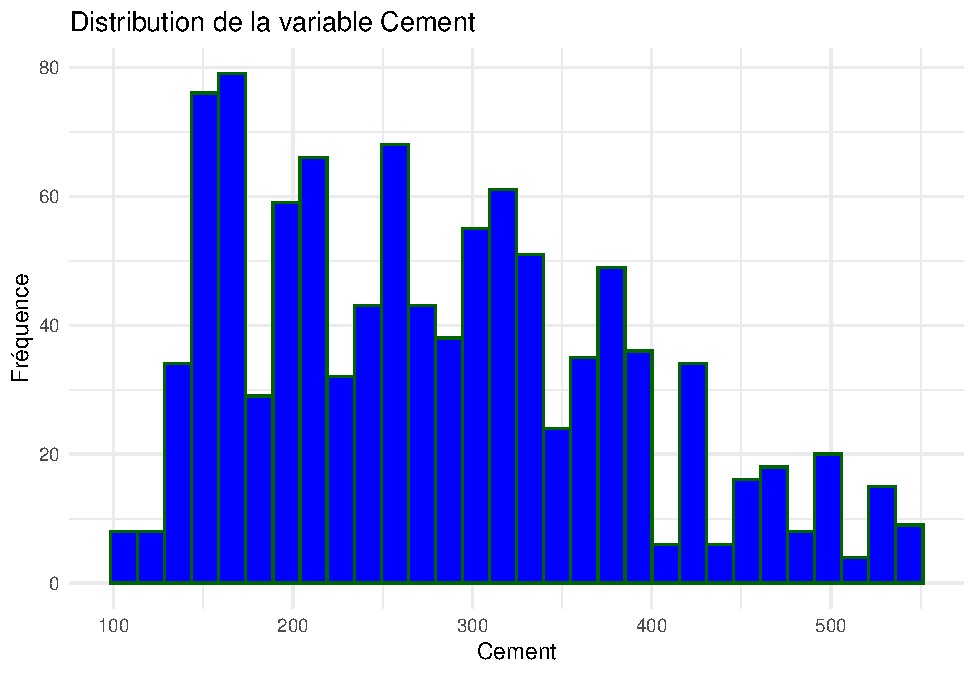
\includegraphics{rmarkdown_airportsv2_files/figure-latex/unnamed-chunk-23-1.pdf}

Nous nous attarderons sur les dimensions 1 et 3 pour effectuer notre
analyse. Cela nous permet de comprendre l'évolution de nos données avec
une vision panoramique et différente de la précédente. En effet,
d'autres variables qui n'ont pas eu d'effet sur les autres dimensions
peuvent s'avérer importantes.

Le troisième axe oppose les grands et moyens aéroports aux autres types
d'aéroports. À ce stade, les moyens aéroports sont très bien représentés
et contribuent énormément à la construction du troisième axe. La Chine,
les États-Unis et les pays classés dans le groupe des ``autres''
contribuent en grande partie à la construction de cet axe. Par
conséquent, nous pouvons conclure que la Chine et les États-Unis
possèdent un nombre important de moyens aéroports.

\begin{verbatim}
## Warning: ggrepel: 10 unlabeled data points (too many overlaps). Consider
## increasing max.overlaps
\end{verbatim}

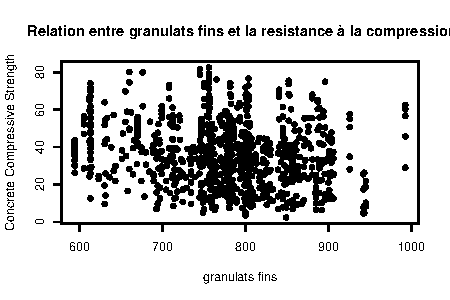
\includegraphics{rmarkdown_airportsv2_files/figure-latex/unnamed-chunk-24-1.pdf}

Nous remarquons à ce niveau que l'analyse se focalise sur le deuxième et
le troisième axe. Nous notons que le Canada et le Brésil expliquent en
grande partie le deuxième axe, d'une part, et que la Chine et les
États-Unis contribuent fortement à l'explication du troisième axe,
d'autre part.

Cela nous permet de comparer les politiques de ces deux pays en termes
d'infrastructures aéroportuaires. La politique aéroportuaire du Canada
et de la Chine répond à des besoins et à des contextes très différents.
Le Canada privilégie une approche flexible et régionale, adaptée à son
vaste territoire et aux particularités géographiques, en utilisant des
solutions comme les hydravions pour desservir les zones isolées. La
Chine, quant à elle, adopte une approche ambitieuse et centralisée pour
développer ses infrastructures, en réponse à une forte demande
intérieure et internationale, en se concentrant sur la construction
rapide de moyens aéroports et la modernisation des infrastructures
existantes pour soutenir sa croissance économique.

\subsection{L'ACP}\label{lacp}

La deuxième partie concerne l'analyse en Composantes Principales (ACP),
qui est une méthode statistique utilisée pour analyser et réduire la
dimensionnalité d'un jeu de données tout en préservant autant que
possible l'information. Elle est souvent utilisée dans des contextes où
les données sont de haute dimension, c'est-à-dire lorsqu'il y a de
nombreuses variables (caractéristiques) qui peuvent être difficiles à
analyser ou à visualiser.

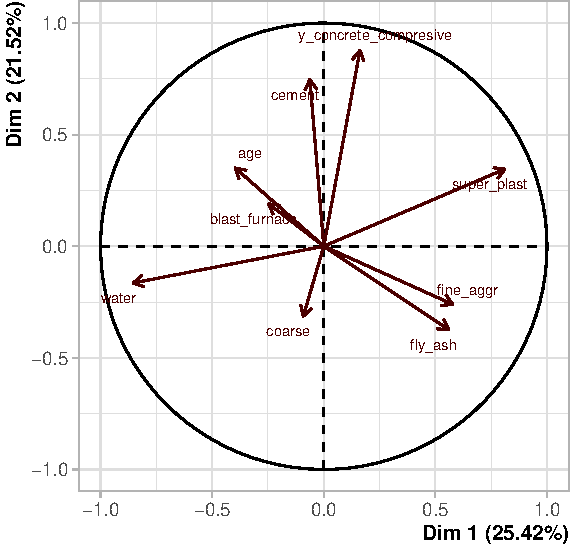
\includegraphics{rmarkdown_airportsv2_files/figure-latex/unnamed-chunk-26-1.pdf}

L'analyse univariée de la variable National Income révèle une
distribution fortement asymétrique, avec la majorité des observations
concentrées dans les tranches de revenu les plus basses. La raison en
est le grand nombre d'aéroports asiatiques présents dans la liste
(Chine, Inde, Philippines). Dans ces pays, le revenu national par
habitant est faible, ce qui contribue à l'asymétrie du graphique. Une
proportion significative du jeu de données se situe entre 20 000 et 60
000, comme le montrent les barres les plus hautes. En revanche, très peu
d'observations dépassent la tranche des 80 000, ce qui met en évidence
une disparité. Cela suggère que la majorité des entités du jeu de
données appartiennent à des pays ou régions ayant des revenus nationaux
modestes, tandis qu'une minorité représente des économies à revenu
élevé.

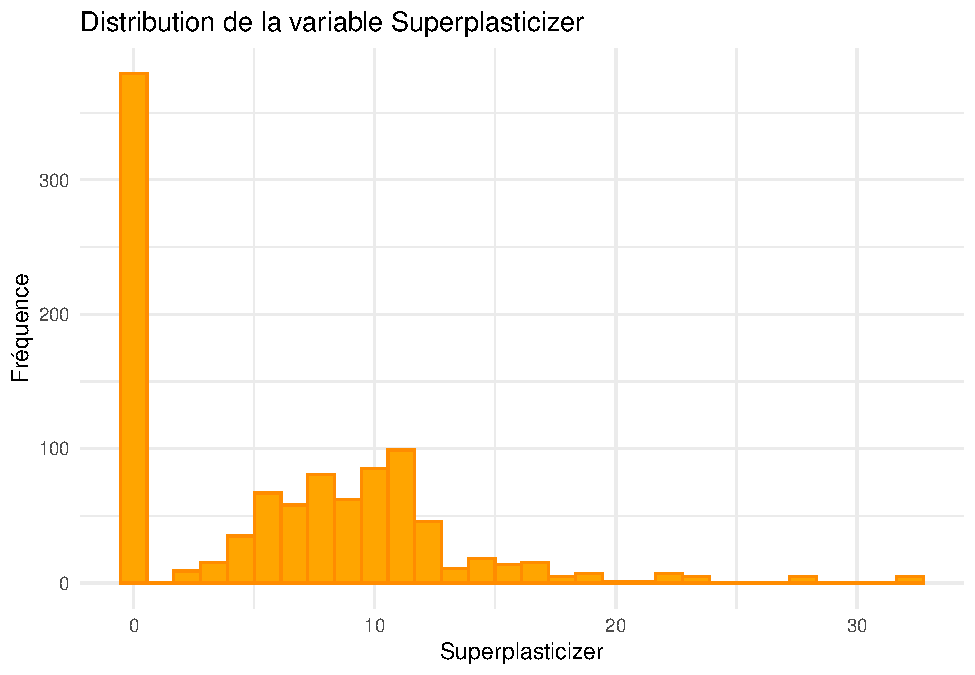
\includegraphics{rmarkdown_airportsv2_files/figure-latex/unnamed-chunk-27-1.pdf}

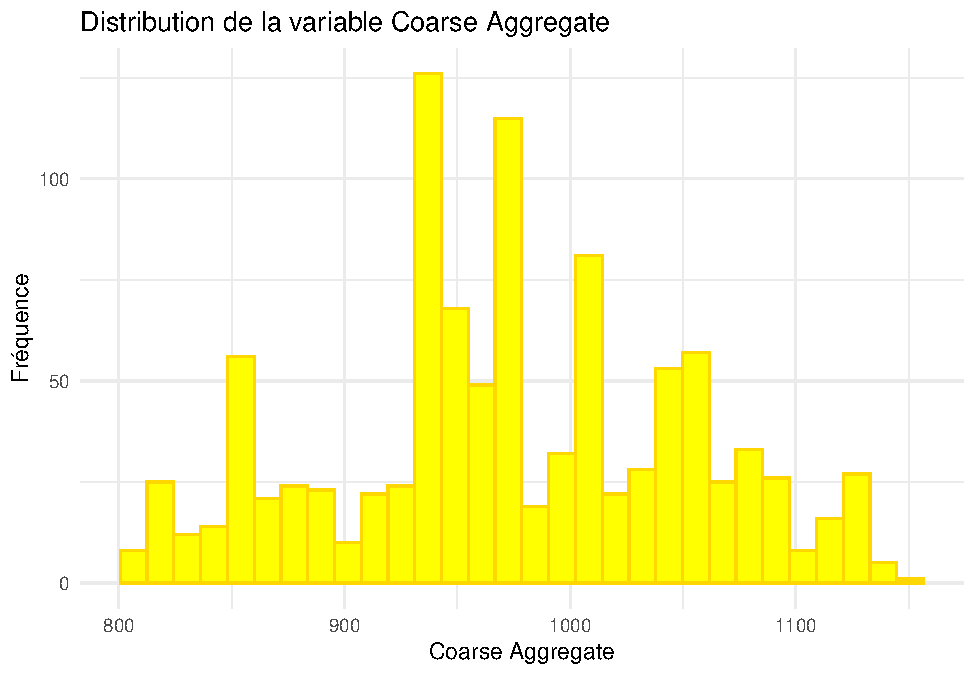
\includegraphics{rmarkdown_airportsv2_files/figure-latex/unnamed-chunk-28-1.pdf}

La comparaison des longueurs de pistes met en évidence une nette
disparité entre les grands aéroports et les petites pistes d'aviation.
Les 50 principaux aéroports disposent de pistes nettement plus longues
et plus homogènes, avec une médiane autour de 11 000 pieds, reflétant
leur capacité à accueillir de grands avions comme les avions
gros-porteurs. En revanche, l'ensemble des 75 052 aéroports montre que
la plupart des pistes sont beaucoup plus courtes, avec une médiane
inférieure à 5 000 pieds, représentant des petits aérodromes régionaux,
privés ou ruraux. Cependant, ce dataset inclut également des valeurs
extrêmes, avec des pistes dépassant les 30 000 pieds, correspondant aux
grands aéroports internationaux. Dans l'ensemble, la distribution est
fortement asymétrique, soulignant la différence entre les petites pistes
et quelques grands hubs internationaux.

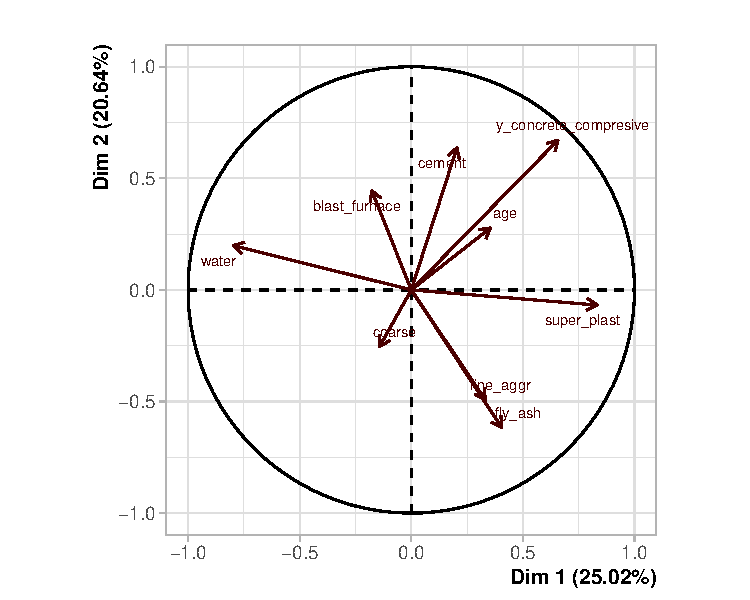
\includegraphics{rmarkdown_airportsv2_files/figure-latex/unnamed-chunk-31-1.pdf}

La matrice de corrélation montre une relation positive forte entre le
revenu national et le nombre de passagers, ce qui suggère que les
aéroports avec un trafic de passagers plus élevé génèrent davantage de
revenus. La longueur des pistes et la largeur des pistes sont fortement
corrélées entre elles, mais n'ont que peu ou pas de relation avec le
revenu national ou le trafic de passagers. Cela indique que, bien que
les dimensions des pistes soient liées entre elles, elles n'influencent
pas directement les revenus ou le flux de passagers. Globalement, le
nombre de passagers semble être le principal moteur du revenu national
pour les aéroports.

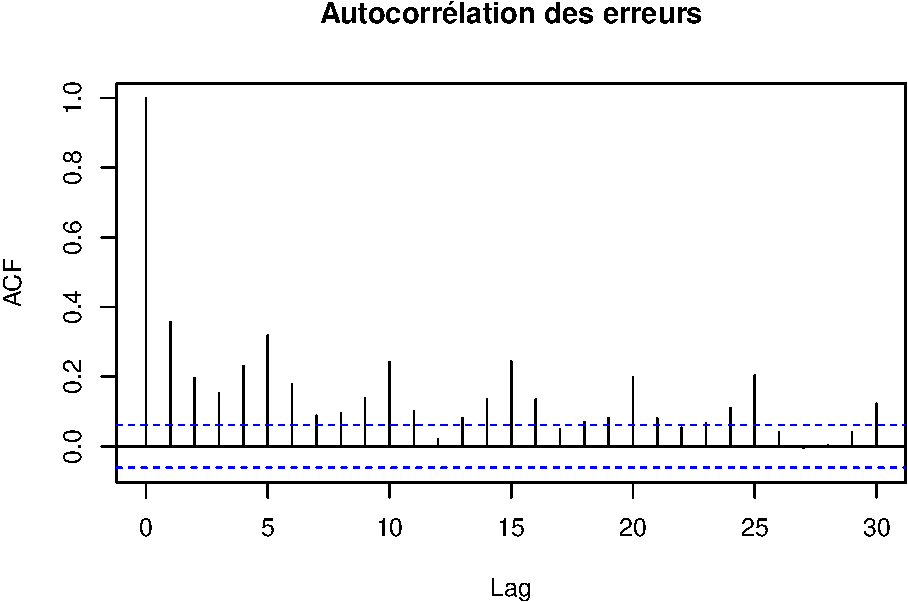
\includegraphics{rmarkdown_airportsv2_files/figure-latex/unnamed-chunk-32-1.pdf}

Le graphique des individus illustre la répartition des observations en
fonction de ces composantes principales. Les points situés dans le
quadrant supérieur droit, comme 27 (Emirats Arabes Unis) et 38
(Singapour), représentent des nations riches avec des infrastructures
avancées et un trafic passagers élevé, reflétant la corrélation positive
entre ces variables. En revanche, des observations comme 6 et 18,
situées dans le quadrant supérieur gauche, correspondent aux États Unis
ayant un revenu modéré mais des infrastructures aéroportuaires atypiques
qui s'écartent de la tendance générale. De manière similaire, des points
comme 43 (La Chine) et 32 (Brésil) dans le quadrant inférieur droit
représentent les pays avec des infrastructures importantes mais des
volumes de passagers faibles.

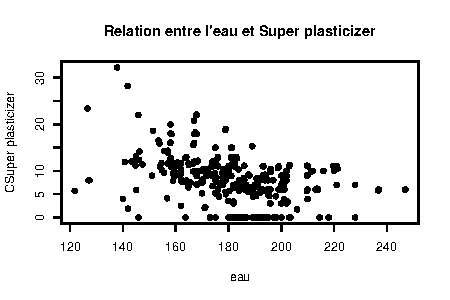
\includegraphics{rmarkdown_airportsv2_files/figure-latex/unnamed-chunk-33-1.pdf}

L'alignement de ``National.income'' avec passengers sur Dim 1 met en
évidence une forte corrélation positive entre la richesse d'un pays et
la demande de transport aérien. En revanche, les vecteurs représentant
la longueur et la largeur des pistes sont étroitement groupés et
orientés principalement sur Dim 2, ce qui suggère que les
caractéristiques physiques des infrastructures sont interdépendantes
mais influencées par des facteurs ne dépendant pas uniquement du revenu
national. Cette séparation entre le trafic passagers lié au revenu et
les caractéristiques physiques des infrastructures implique que, bien
que les pays riches investissent généralement dans des aéroports plus
grands et mieux équipés, l'expansion des infrastructures n'est pas
toujours proportionnelle aux niveaux de revenu.

\begin{verbatim}
##        eigenvalue percentage of variance cumulative percentage of variance
## comp 1  1.5104137               37.76034                          37.76034
## comp 2  1.2527188               31.31797                          69.07831
## comp 3  0.7158910               17.89728                          86.97559
## comp 4  0.5209765               13.02441                         100.00000
\end{verbatim}

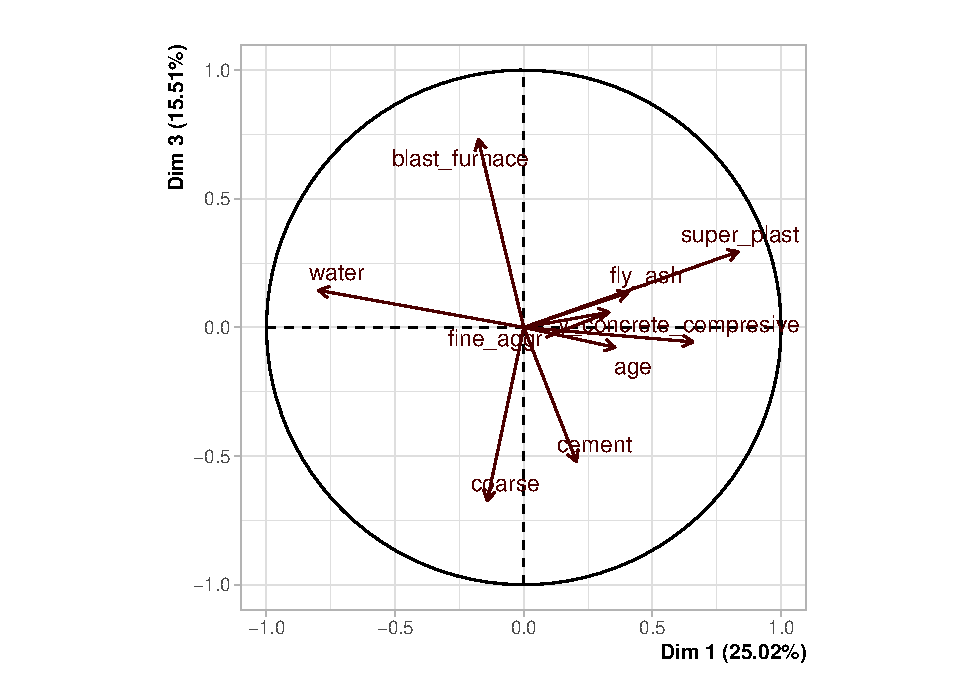
\includegraphics{rmarkdown_airportsv2_files/figure-latex/unnamed-chunk-34-1.pdf}

L'histogramme des valeurs propres montre la contribution des quatre
composantes principales (comp 1, comp 2, comp 3 et comp 4) à
l'explication de la variance dans le jeu de données. La composante 1
capture la majeure partie de la variance, révélant les principales
structures des données (comme le revenu national, le volume de passagers
ou les dimensions des pistes). La composante 2 contribue également de
manière significative, bien qu'à un degré moindre, en expliquant des
variations complémentaires. En revanche, les composantes 3 et 4 ont des
contributions nettement plus faibles, indiquant qu'elles expliquent des
variations mineures. Cela suggère que les deux premières composantes
suffisent pour représenter la majorité des informations du jeu de
données tout en simplifiant l'analyse et la visualisation.

\section{\texorpdfstring{\textbf{Source}}{Source}}\label{source}

Airports :
\url{https://www.kaggle.com/datasets/danishjmeo/world-airports-data}

Top airports :
\url{https://en.wikipedia.org/wiki/List_of_busiest_airports_by_passenger_traffic}

ISO codes :
\url{https://en.wikipedia.org/wiki/List_of_ISO_3166_country_codes}

National Income : \url{https://wid.world/data/}

\end{document}
